%#! platex %f && dvipdfmx -d 5 tougetsuan191111journalclub
%
%
% $B<j$G!$%3%s%Q%$%k$9$kJ}K!(B
% platex tougetsuan180205a
% pbibtex tougetsuan180205a
% platex tougetsuan180205a
% dvipdfmx -d 5 tougetsuan180205a
%
\documentclass[a4paper,twocolumn,twoside,10pt]{jarticle}
\usepackage{nidanfloat} %% add
\usepackage{graphics}
\usepackage[dvips,usenames]{color}  % for revise color
\usepackage{graphicx}
\usepackage{plain}
\usepackage{fancyhdr}
\pagestyle{fancyplain}
\usepackage{amssymb}
\usepackage{bm}
\usepackage{float}
%$B%U%m!<%H4D6-$H$=$NA08e$NK\J8$H$N%9%Z!<%9(B
\setlength\floatsep{0pt} %$B%Z!<%8>eIt$"$k$$$O2<It$K=PNO$5$l$k%U%m!<%H$H%U%m!<%H$N4V$N5wN%(B
\setlength\intextsep{8pt} %$B%Z!<%8$NESCf$K=PNO$5$l$k%U%m!<%H$H$=$NA08e$NK\J8$H$N5wN%(B
%\setlength\textfloatsep{0pt} %$B%Z!<%8>eIt$N%U%m!<%H$HK\J8!$$*$h$SK\J8$H(B
%$B%Z!<%82<It$N%U%m!<%H$H$N5wN%(B
\setcounter{page}{13}
\topmargin = -15mm
\oddsidemargin = 0mm
\evensidemargin = -10mm
\textwidth = 162mm
\textheight = 250mm
\columnsep = 10mm
\renewcommand{\footrulewidth}{0pt}
\renewcommand{\headrulewidth}{0pt}
\bmdefine{\bx}{x}



\begin{document}
\lhead{}
\rhead{}
\rhead{2019$BG/(B11$B7n(B12$BF|(B}
% \begin{twocolumn}
\twocolumn[
\begin{center}
 {\large
 \newblock
 {\gt $B>pJs9)3X%;%_%J!<(B $BO@J8>R2p(B} \vspace{5mm}\\
P.~{F\"{o}ldi\'{a}k}. \\
 Learning invariance from transformation sequences\\
\newblock {\em Neural Computation}, 3:194--200, 1991.
 }
\vspace{3mm}  \\
% {\large $B5\:jBg3X!!9)3XIt!!>pJs%7%9%F%`9)3X2J(B}\vspace{2mm} \\
{\large $BH/I=<T!'(B 67140770  $BEm7n0C(B $B$"$i$l(B} \vspace{10mm}\\
\end{center}]

%\input{titles}
\section{$B$O$8$a$K(B}

$B!;!;!J$3$s$JLLGr$$LdBj$,$"$k!K!%(B
$B!;!;(B
$B!J$=$NLdBj$KBP$7$F$3$l$^$G$I$s$J8&5f$,$J$5$l$F$-$?$+!$8&5f$NNr;K$rDI$&!K!%(B
$B$7$+$7!$$3$s$J!J4JC1$J!K$3$H$bJ,$+$C$F$$$J$$(B
$B!J$^$@8&5f$OIT==J,!%$3$NE@$,J,$+$C$F$$$J$$!%$3$l$,2r7h$G$-$l$P!*!K!%(B
$B$@$+$i!$:#2s$3$NO@J8$NCx<T$O!$$3$s$J<B83$r$7$?!J;v<B!K!%(B
$B$=$l$G!$$3$s$J7k2L$,F@$i$l$?!J;v<B!K!%(B
$B$3$N7k2L$O(B $B!{!{!{$G$"$k$3$H$r!V<(:6!W$7$F$$$k!J;v<B$G$O$J$$!#Cx<T$N0U8+!"(B
$BM=A[!K$HCx<T$O<gD%$7$F$$$k!%(B

  % $B$O$8$a$K(B
\section{神経回路モデルと学習手法}
ここは手法.

\subsection{誤差逆伝播法}
スペースの都合上,説明は省略する.
  % $B<jK!(B
%\rhead{}
%\input{experiment}  % $B<B83(B
\section{結果}
% --- experiment.tex から移動 ここから
\subsection{一層目の重みの学習}
\begin{figure}[hbt]
\centering
\begin{minipage}{0.45\columnwidth}
  \centering
  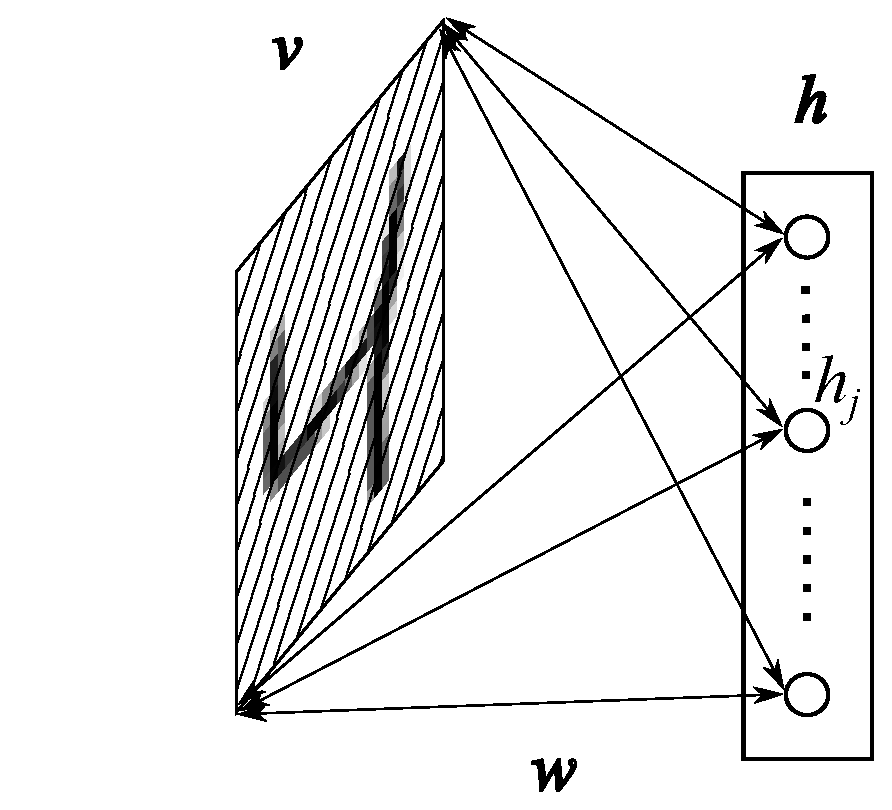
\includegraphics[width=0.8\columnwidth]{lookall_network_v7.eps}
  \caption{実験1のRBM}
  \label{cap:lookall_network}
\end{minipage}
\begin{minipage}{0.45\columnwidth}
  \centering
  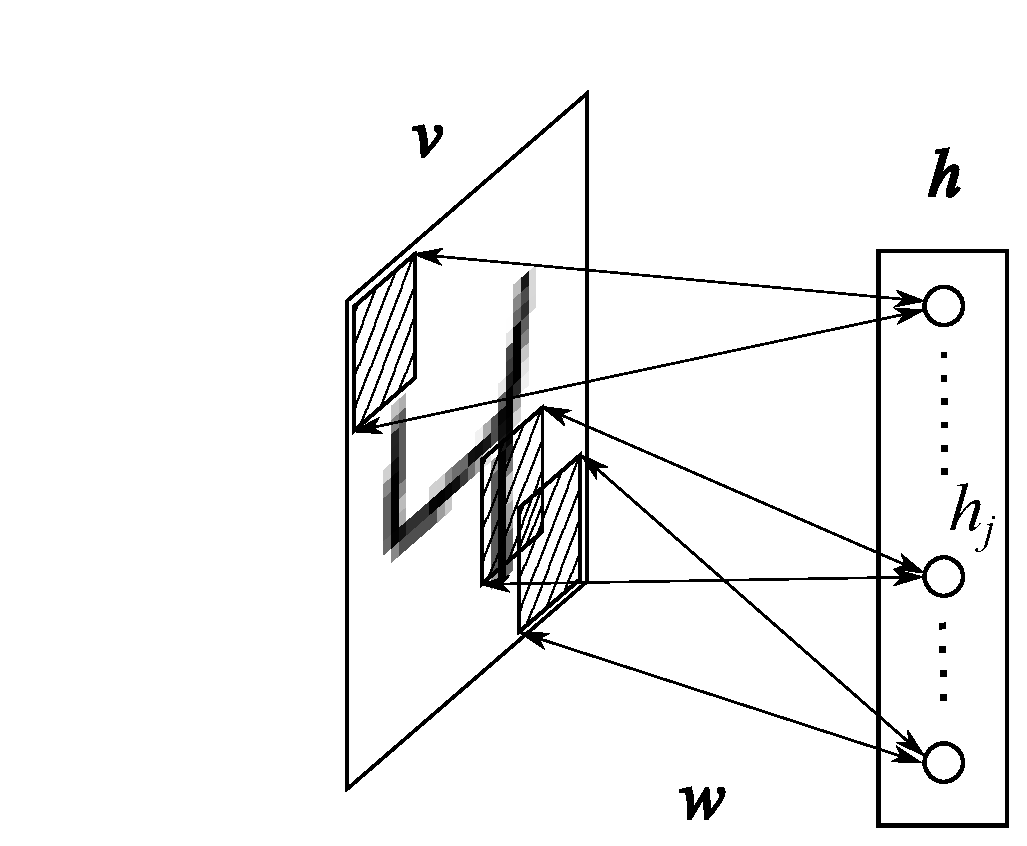
\includegraphics[width=0.9\columnwidth]{lookpartial_network_v8.eps}
  \caption{実験2のRBM}
  \label{cap:lookpartial_network}
\end{minipage}
\end{figure}
\subsubsection{実験1}
%\subsubsection{隠れ層1の素子と可視層の素子が全て結合しているRBM}
図~\ref{cap:lookall_network}のような,
可視層が$784$次元,隠れ層が$500$次元のRBMにて
手書き文字2000枚を用いて
学習率$0.001$で$1000$回の学習をした.
隠れ層の素子${h_j}$は,図~\ref{cap:lookall_network}の斜線で示した
可視層の素子$v_i$すべてと結合している.
\begin{table}%[htb]
\begin{center}
  \caption{各実験における正答率}
  \label{tab:result}
  \begin{tabular}{cccc}
    \hline
    実験   & Training set & Test set\\
    \hline \hline
    実験1  & 89.08\%      & 88.69\% \\
    実験2  & 87.34\%      & 88.36\% \\
    実験3  & 91.86\%      & 91.55\% \\
    \hline
  \end{tabular}
\end{center}
\end{table}

  % $B7k2L(B
%\input{summary}  % $BMWLs(B


%%%% $B;29MJ88%(B %%%

\section{$B;29MJ88%$N=q$-J}(B}
$B;29MJ88%$O!$(B
$BK\J8Cf$GI,$:0zMQ$9$k(B\cite{hopfield83a}$B!%(B
$BK\J8$G0zMQ$7$F$$$J$$$b$N$r(B
$B;29MJ88%$N%j%9%H$K$O5-=R$7$J$$(B\cite{foldiak91a,sgeman88a,sabour2017a}$B!%(B

\bibliographystyle{jabbrv}
% \bibliographystyle{sieicej}
\bibliography{irl_bibs_2019.bib}


% \rhead{}  % 2$BKgL\0J9_$KF|IU$,=P$J$$$h$&$K$9$k!%(B
\end{document}
